%
% Latex example file for postgrads (04/10/03)
%
% If you have questions please email me: 
%
% M.L.Balogh@durham.ac.uk
%
% or find me in room OC312.
%
% you can copy this file and others from :
%
% http://star-www.dur.ac.uk/~balogh/latex/
%
% Note you can get Latex style files etc. from http://www.ctan.org

% Latex2e style  declaration


% The emulateapj.cls file produces output like that of the
% Astrophysical Journal.  Use instead of aastex.cls.  This usage
% supercedes older versions that used the aastex package with emulateapj5.sty.
% YOU SHOULD REMOVE THE TABLE OF
% CONTENTS PAGE WHEN USING APJ FORMAT.
%
\documentclass[11pt,a4paper]{emulateapj}
\bibliographystyle{apj}


%define general packages
\usepackage{epsfig}
\usepackage{amsmath}
\usepackage{natbib}

%internal short cuts
\def \HgA {H$\gamma_A$}
\def \gon {Gonz\'{a}lez}
\def \Hbp {H$\beta ^\prime$}

\begin{document}

\title{COMPLETE View of the Ophiuchus Cloud I: Stellar Wind Driven by B-type Stars}
\author{Hope Chen \& Aaron Meisner}
\date{\today}
%\maketitle


% Usually omit these for ApJ or MNRAS style files:
%\tableofcontents
%
%\listoffigures
%
%\listoftables

\begin{abstract}
\textbf{Abstract} Using data from the COordinated Molecular Probe Line
Extinction Thermal Emission (COMPLETE) Survey of Star Forming Regions
and the complementary data from the Herschel Gould Belt Survey, we
present an analysis of three different column density tracers --
near-infrared extinction, far-infrared dust thermal emission, and
molecular line emission of the \textsuperscript{12}CO J=1-0 and
\textsuperscript{13}CO J=1-0 transitions. In this paper, we compare
column densities based on these three different tracers and try to
provide a prescription for tracing material in various parts of a
molecular cloud. Based on the derived column density and temperature, we
report a shell-like structure that is potentially the result of an
embedded B-star wind. We also examine the variation of the column
density probability distribution function (PDF) across the Ophiuchus
cloud. This is further compared with the information of the cloud
dynamics derived from the \textsuperscript{12}CO and
\textsuperscript{13}CO data. We conclude that one needs to take extreme
care when tracing the column density structure and interpreting its
relation with the dynamics in a molecular cloud. A detailed simulation
with proper synthetic observation is required to explain the
(non-)correlation between the column density PDF and the turbulence
(represented by the Mach number) in the Ophiuchus cloud.

\end{abstract}

%Section heading
\section{Introduction}
\label{sec:introduction}
Nearby Gould Belt Clouds are often targets of star formation observations. Their small distances from the Earth provide astronomers a chance to resolve the star formation activities. The first step to understand the environment of star formation in these clouds is to trace their mass structures. To do so, people often employ three different kinds of methods: molecular line emission, extinction of background stars by the dust in the clouds, and the dust thermal emission in the mid/far-infrared wavelengths.
The first observation of molecular line emission from star forming regions dates back to [????] (Ref?). Observation of line emission provides information of the line-of-sight velocity.
The extinction of background stars corresponds to the amount of dust material 

\section{Data}
\label{sec:data}
In this paper, we use data from the COordinated Molecular Probe Line Extinction Thermal Emission (COMPLETE) Survey of Star Forming Regions. Together with data from a broader collaboration, these include 1) an extinction map based on near-infrared data from the Two Micron All-Sky Survey (2MASS) and a near-infrared color excess method, the NICEST algorithm \citep[][note that this is an improved version of the NICER algorithm and is developed after the COMPLETE Survey]{Lombardi_2009}, 2) 60 and 100 $\mu$m maps from the Improved Reprocessing of the IRAS data \citep[IRIS;]{Miville_Deschenes_2005}, and 3) the molecular line emission of the $^{12}$CO J=1-0 and $^{13}$CO J=1-0 transitions obtained at the Five College Radio Astronomy Observatory (FCRAO). We also include archival Herschel data, which were taken as part of the Herschel Gould Belt Survey. The Herschel data allow us to derive column density and other physical properties based on the more complete SED of far-infrared dust thermal emission than the 60 and 100 $\mu$m bands of the IRIS data.

\subsection{2MASS/NICEST Extinction}
The NICEST algorithm is the latest version of a near-infrared color excess method to derive the dust extinction based on near-infrared observation. Its predecessors include the NICE and the NICER algorithms \citep{Lombardi_2001,Lombardi_2005}.

\subsection{IRAS/IRIS 60 and 100 $\mu$m maps}
The Infrared Astronomical Satellite (IRAS) performed a survey that covered 98 \% of the sky at four wavelenths: 12, 25, 60, and 100 $\mu$m \citep{Neugebauer_1984}. However, the widely used dataset released in 1994 (IRAS Sky Survey Atlas; Wheelock and Infrared Processing and Analysis Center, 1994) suffers from the calibration, zero level, and striping problems. The Improved Reprocessing of the IRAS data \citep[IRIS;]{Miville_Deschenes_2005} provides a significant improvement over these problems. For the purpose of this paper, we use only the 60 and 100 $\mu$m maps of the Ophiuchus region from the IRIS data product and a simple two-band method similar to that used by \citet{Schnee_2008} to derive the column density for the Perseus molecular cloud (see the next section).

\begin{figure*}[ht]
\centering
%% The 'scale' parameter below allows you to scale the figure so that it fits within the page. In this case the figure was scaled to 20% of its original size. Note: for .png files one has to use pdflatex, not classic latex
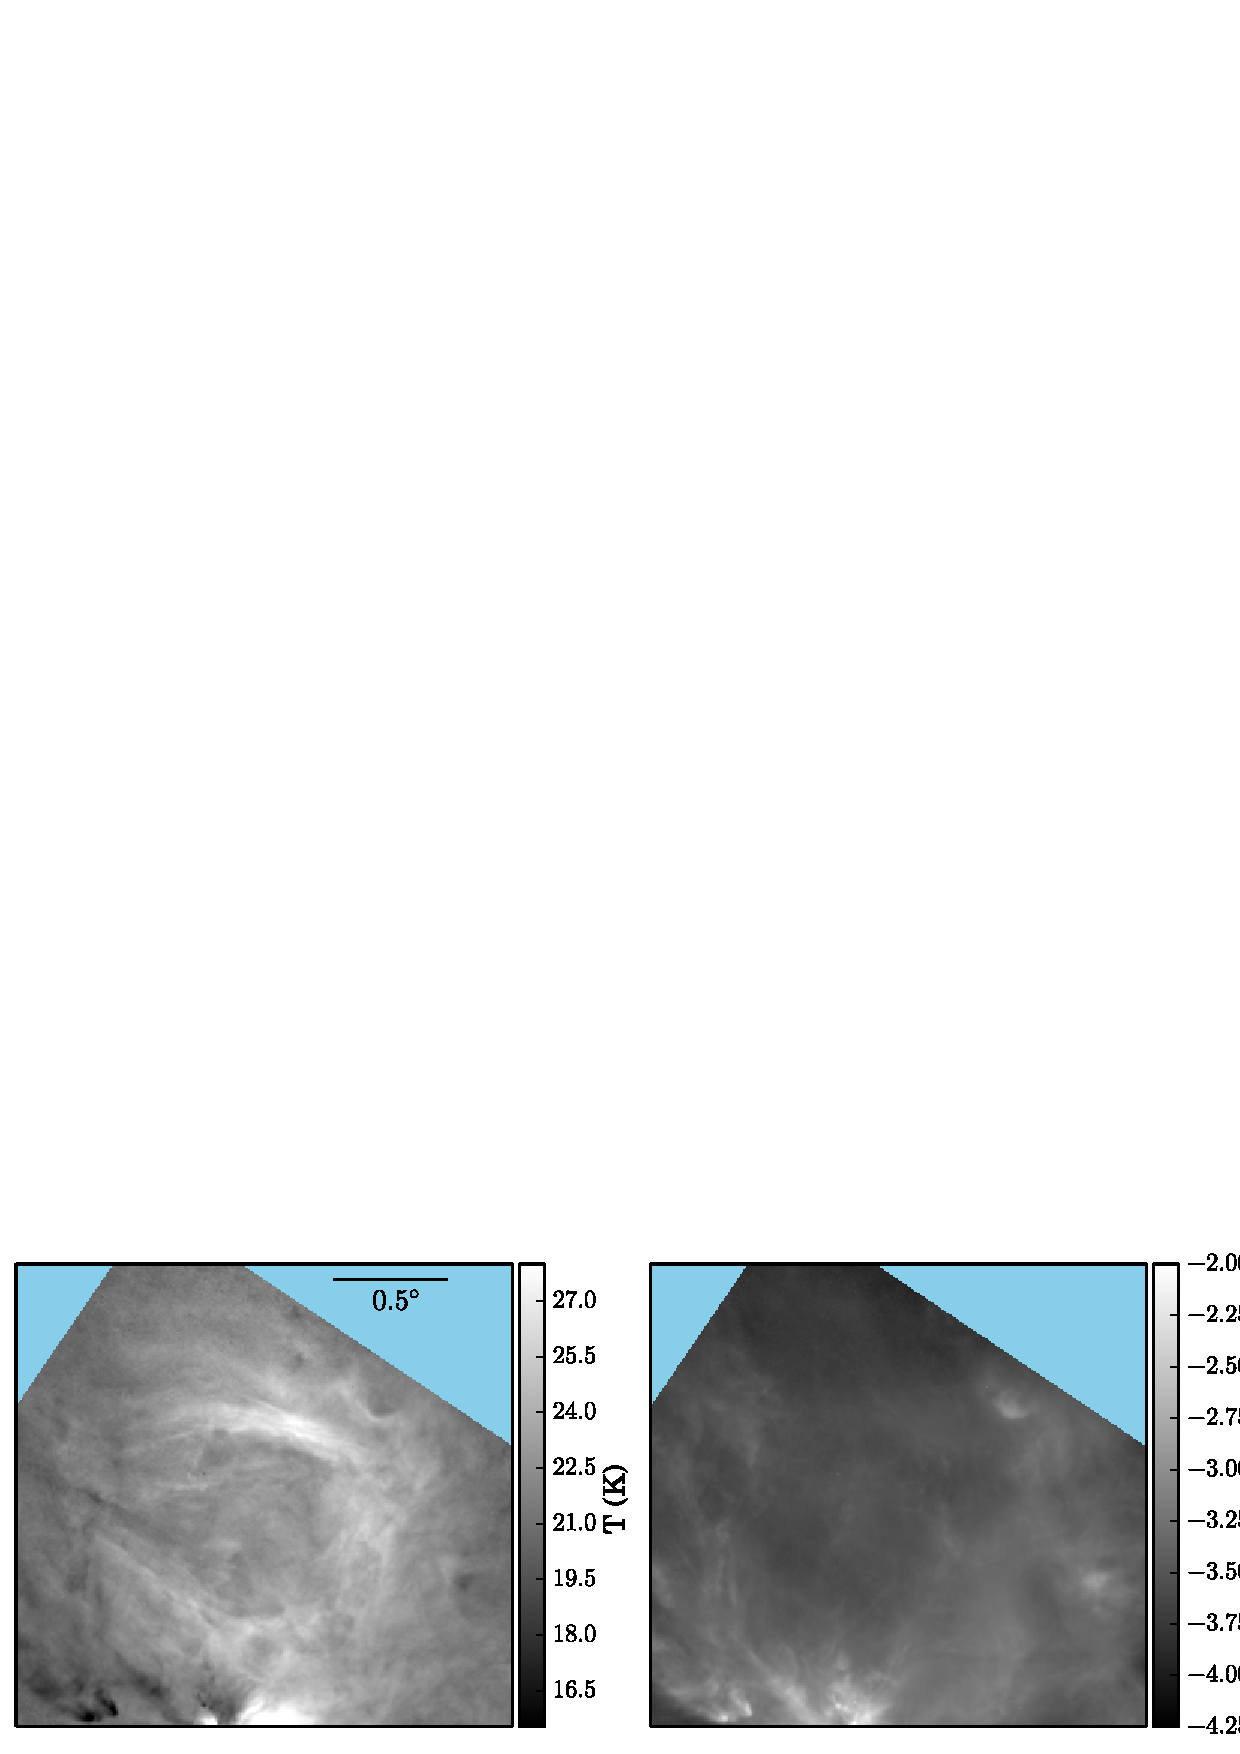
\includegraphics[scale=0.8]{fig/shell_herschel.png}
\caption{The image shows \textit{Herschel}-based temperature and opacity at 350 $\mu$m.
}
\end{figure*}

\subsection{Herschel Archival Data}
The Herschel Space Observatory was a satellite operated by the European Space Agency. Its Photodetecting Array Camera and Spectrometer (PACS) and Spectral and Photometric Imaging Receiver (SPIRE) covered wavelengths from 55 to 670 $\mu$m, with six wide spectral bands: 70, 100, and 160 $\mu$m bands of PACS and 250, 350, and 500 $\mu$m bands of SPIRE. A wide range of the Herschel data products is availabel in the Herschel Science Archive. In this paper, we use data that were obtained as part of the Herschel Gould Belt Survey \citep{Andr__2010}. The maps presented in this paper are produced in the Herschel Interactive Processing Environment (HIPE; Version 11.1.0 was used to produce these maps). The zero level problem is resolved by comparing the maps with predictions from the two-component dust model fitted to the Planck HFI maps of the Ophiuchus region (Meisner \& Finkbeiner, submitted; ArXiv:1410.7523). Again, for the purpose of this paper, only maps of the longest four wavelengths (160 $\mu$m of PACS and 250/350/500 $\mu$m of SPIRE) are used here, since emission at wavelengths shorter than 100 $\mu$m shows significant contribution from emission of ``very small grains (VSGs)'' and requires a dust model more complicated than described by Meisner \& Finkbeiner (submitted). The same situation applies to the IRIS 60 and 100 $\mu$m maps, and an estimate of error is given by \citet{Schnee_2006} and \citet{Schnee_2007}.

\subsection{Molecular Line Emission: $^{12}$CO (1-0) and $^{13}$CO (1-0)}
Observations of molecular line emission of the $^{12}$CO J=1-0 and $^{13}$CO J=1-0 transitions were carried out at the 14m Five College Radio Astronomy Observatory \citep[FCRAO;]{Ridge_2006}. The SEQUOIA 32-element focal-plane array was used to make an on-the-fly map of the Ophiuchus region. A total bandwidth of 25 MHz with 1024 channels in each IF in the dual-IF mode yielded an effective velocity resolution of 0.07 km s$^{-1}$. This allows us to resolve subsonic velocity structures in a typical molecular cloud environment \citep[with a temperature of 15 K and an average molecular weight of 2.33 m$_H$;]{Carey_1998,Pillai_2006}.

\section{Methods}
\label{sec:methods}
Figure 1 shows the column densities based on the data described in Section \ref{sec:data}. For comparison, column densities are converted to the unit of V-band extinction (A$_V$) using a uniform conversion factor of N(H$_2$)/A$_V$ = 6.9 $\times$ 10$^{20}$ cm$^{-2}$ mag$^{-1}$ \citep{Draine_2003,Evans_2009}. (Different factors were suggested for more diffuse regions, for example, N(H$_2$)/A$_V$ = 9.4 $\times$ 10$^{20}$ cm$^{-2}$ mag$^{-1}$ by \citet{Bohlin_1978}.) For the 2MASS/NICEST extinction map, we assume a linear reddening law of A$_K$/A$_V$ = 0.114. Besides the column density, other physical properties including the temperature are derived from these data based on respective assumptions described as follows.

\subsection{Modeling far-infrared emission with a single-component modified blackbody equation}
For both the IRIS and the Herschel data, we assume that the emission at respective wavelengths (60 and 100 $\mu$m for the IRIS maps, and 160/250/350/500 $\mu$m for the Herschel PACS and SPIRE maps) is dominated by the ``big grain \citep[BG;]{Stepnik_2003}'' dust thermal emssion. We also assume that the dust thermal emission can be described by a single-component modified blackbody equation. This assumption is true only on certain conditions and can be a very coarse approximation at wavelengths shorter than 100 $\mu$m. This is because that the emission at wavelengths shorter than 100 $\mu$m starts to see ``contamination'' from the VSG emission. \citet{Schnee_2007} examined this effect and gave an estimate of error for a similar method to derive the column density and dust temperature. They conluded that the typical error at 60 $\mu$m is around 20\% and smaller for longer wavelengths. Since our goal here is to provide a a relative comparison of the IRIS and the Herschel data, using maps of emission at the longest two of the IRAS wavelengths suffices.


\subsubsection{Temperature and column density from the Herschel data}
Similarly, we assume that the emission at Herschel PACS 160 $\mu$m and SPIRE 250/350/500 $\mu$m bands is dominated by the dust thermal emission and can be described by a single modified blackbody equation. This is a better assumption for the Herschel data used in this paper, since the VSG emission shows up mostly at wavelengths shorter than 100 $\mu$m.

\subsubsection{Modeling far-infrared emission with a single-component modified blackbody equation}
Using a single-component modified blackbody equation presumes that the material along the line of sight has a single temperature.

Finally, as \citet{Finkbeiner_1999} and Meisner \& Finkbeiner (submitted; ArXiv:1410.7523) suggested, the modeling is improved by using a two-compoenent modified blackbody equation with a ``hot dust component'' and a ``cold dust component.'' The emission is then described by the equation:

By comparing the two-component model to the single-component model, Meisner \& Finkbeiner (submitted) found that the single-component modified blackbody equation generally underpredicts dust emission at all Planck spectral bands from 100 to 3000 GHz (2 mm to 67 $\mu$m). This is consistent with our analysis above.

Although the wavelength range suggested by Meisner \& Finkbeiner where one should adopt the two-component model covers the two IRAS wavelengths (60 and 100 $\mu$m) and the four Herschel wavelengths (160, 250, 350, and 500 $\mu$m) conisdered in this paper, we use a single modified blackbody equation in consistency with works done by the Gould Belt Survey team. Analysis of the two-component model is beyond the scope of this paper.

\subsubsection{Temperature-spectral index anti-correlation and a Bayesian solution}

\citet{Kelly_2012} suggested a solution to the artificial anti-correlation between the temperature and the spectral index, using a hierarchical Bayesian method.

However, the hierarchical Bayesian method is highly computation-expensive. Assuming a linear law between the computation time and the number of pixels on the map, we estimate the total computation time of one month to finish the calculation of the column density and temperature using the hierarchical Bayesian method, for a map as large as the Herschel maps of the Ophiuchus cloud in Figure 1.

\subsection{Column density from $^{12}$CO (1-0) and $^{13}$CO (1-0) emission}
We follow the steps taken by \citet{Pineda_2008} to derive

\subsection{Column density probability distribution function (PDF)}


\section{Results}
\label{sec:results}

\begin{figure}[ht]
\centering
%% The 'scale' parameter below allows you to scale the figure so that it fits within the page. In this case the figure was scaled to 20% of its original size. Note: for .png files one has to use pdflatex, not classic latex
\includegraphics[scale=0.35]{fig/shell_2mass.png}
\caption{The shell region on top of the NICEST extinction map.
}
\end{figure}

\begin{figure*}[ht]
\centering
%% The 'scale' parameter below allows you to scale the figure so that it fits within the page. In this case the figure was scaled to 20% of its original size. Note: for .png files one has to use pdflatex, not classic latex
\includegraphics[scale=0.5]{fig/v_exp}
\caption{The expanding velocity of the shell, derived from FCRAO $^{12}CO$ data.
}
\end{figure*}

\begin{figure}[ht]
\centering
%% The 'scale' parameter below allows you to scale the figure so that it fits within the page. In this case the figure was scaled to 20% of its original size. Note: for .png files one has to use pdflatex, not classic latex
\includegraphics[scale=0.35]{fig/bar_energy.png}
\caption{Energy comparison between the shell and the clouds.
}
\end{figure}

\subsection{Column density ``calibration'' and comparison}

\subsection{Shell-like structure centered at the B-type star, $\rho$ Ophiuchi}

\subsection{Column density distributions across the Ophiuchus cloud}

\subsubsection{Column density PDF and turbulence}

\subsubsection{Column density PDF and star formation}

\section{Discussion}
\label{sec:discussion}

\subsection{Column density tracers: when to use what}

\subsection{Shell-like structure: an embedded B-star wind?}

\subsection{(Non-)Correlation between column density distribution and the dynamics in a molecular cloud}

\section{Summary}
\label{sec:summary}

\begin{enumerate}
\item The three tracers
\item Problems with Herschel, and (im)possible solution using the Bayesian method
\item Column density distribution and its characterization
\item Column density distribution and dynamics in the Ophiuchus cloud
\end{enumerate}

%\bibliography{bibliography/converted_to_latex.bib%
%}

\bibliographystyle{apj}
\bibliography{oph_shell}

\end{document}
